% Options for packages loaded elsewhere
\PassOptionsToPackage{unicode}{hyperref}
\PassOptionsToPackage{hyphens}{url}
\PassOptionsToPackage{dvipsnames,svgnames,x11names}{xcolor}
%
\documentclass[
  letterpaper,
  DIV=11,
  numbers=noendperiod]{scrartcl}

\usepackage{amsmath,amssymb}
\usepackage{iftex}
\ifPDFTeX
  \usepackage[T1]{fontenc}
  \usepackage[utf8]{inputenc}
  \usepackage{textcomp} % provide euro and other symbols
\else % if luatex or xetex
  \usepackage{unicode-math}
  \defaultfontfeatures{Scale=MatchLowercase}
  \defaultfontfeatures[\rmfamily]{Ligatures=TeX,Scale=1}
\fi
\usepackage{lmodern}
\ifPDFTeX\else  
    % xetex/luatex font selection
\fi
% Use upquote if available, for straight quotes in verbatim environments
\IfFileExists{upquote.sty}{\usepackage{upquote}}{}
\IfFileExists{microtype.sty}{% use microtype if available
  \usepackage[]{microtype}
  \UseMicrotypeSet[protrusion]{basicmath} % disable protrusion for tt fonts
}{}
\makeatletter
\@ifundefined{KOMAClassName}{% if non-KOMA class
  \IfFileExists{parskip.sty}{%
    \usepackage{parskip}
  }{% else
    \setlength{\parindent}{0pt}
    \setlength{\parskip}{6pt plus 2pt minus 1pt}}
}{% if KOMA class
  \KOMAoptions{parskip=half}}
\makeatother
\usepackage{xcolor}
\setlength{\emergencystretch}{3em} % prevent overfull lines
\setcounter{secnumdepth}{5}
% Make \paragraph and \subparagraph free-standing
\ifx\paragraph\undefined\else
  \let\oldparagraph\paragraph
  \renewcommand{\paragraph}[1]{\oldparagraph{#1}\mbox{}}
\fi
\ifx\subparagraph\undefined\else
  \let\oldsubparagraph\subparagraph
  \renewcommand{\subparagraph}[1]{\oldsubparagraph{#1}\mbox{}}
\fi


\providecommand{\tightlist}{%
  \setlength{\itemsep}{0pt}\setlength{\parskip}{0pt}}\usepackage{longtable,booktabs,array}
\usepackage{calc} % for calculating minipage widths
% Correct order of tables after \paragraph or \subparagraph
\usepackage{etoolbox}
\makeatletter
\patchcmd\longtable{\par}{\if@noskipsec\mbox{}\fi\par}{}{}
\makeatother
% Allow footnotes in longtable head/foot
\IfFileExists{footnotehyper.sty}{\usepackage{footnotehyper}}{\usepackage{footnote}}
\makesavenoteenv{longtable}
\usepackage{graphicx}
\makeatletter
\def\maxwidth{\ifdim\Gin@nat@width>\linewidth\linewidth\else\Gin@nat@width\fi}
\def\maxheight{\ifdim\Gin@nat@height>\textheight\textheight\else\Gin@nat@height\fi}
\makeatother
% Scale images if necessary, so that they will not overflow the page
% margins by default, and it is still possible to overwrite the defaults
% using explicit options in \includegraphics[width, height, ...]{}
\setkeys{Gin}{width=\maxwidth,height=\maxheight,keepaspectratio}
% Set default figure placement to htbp
\makeatletter
\def\fps@figure{htbp}
\makeatother

\usepackage{booktabs}
\usepackage{longtable}
\usepackage{array}
\usepackage{multirow}
\usepackage{wrapfig}
\usepackage{float}
\usepackage{colortbl}
\usepackage{pdflscape}
\usepackage{tabu}
\usepackage{threeparttable}
\usepackage{threeparttablex}
\usepackage[normalem]{ulem}
\usepackage{makecell}
\usepackage{xcolor}
\usepackage{siunitx}

  \newcolumntype{d}{S[
    input-open-uncertainty=,
    input-close-uncertainty=,
    parse-numbers = false,
    table-align-text-pre=false,
    table-align-text-post=false
  ]}
  
\KOMAoption{captions}{tableheading}
\makeatletter
\makeatother
\makeatletter
\makeatother
\makeatletter
\@ifpackageloaded{caption}{}{\usepackage{caption}}
\AtBeginDocument{%
\ifdefined\contentsname
  \renewcommand*\contentsname{Table of contents}
\else
  \newcommand\contentsname{Table of contents}
\fi
\ifdefined\listfigurename
  \renewcommand*\listfigurename{List of Figures}
\else
  \newcommand\listfigurename{List of Figures}
\fi
\ifdefined\listtablename
  \renewcommand*\listtablename{List of Tables}
\else
  \newcommand\listtablename{List of Tables}
\fi
\ifdefined\figurename
  \renewcommand*\figurename{Figure}
\else
  \newcommand\figurename{Figure}
\fi
\ifdefined\tablename
  \renewcommand*\tablename{Table}
\else
  \newcommand\tablename{Table}
\fi
}
\@ifpackageloaded{float}{}{\usepackage{float}}
\floatstyle{ruled}
\@ifundefined{c@chapter}{\newfloat{codelisting}{h}{lop}}{\newfloat{codelisting}{h}{lop}[chapter]}
\floatname{codelisting}{Listing}
\newcommand*\listoflistings{\listof{codelisting}{List of Listings}}
\makeatother
\makeatletter
\@ifpackageloaded{caption}{}{\usepackage{caption}}
\@ifpackageloaded{subcaption}{}{\usepackage{subcaption}}
\makeatother
\makeatletter
\@ifpackageloaded{tcolorbox}{}{\usepackage[skins,breakable]{tcolorbox}}
\makeatother
\makeatletter
\@ifundefined{shadecolor}{\definecolor{shadecolor}{rgb}{.97, .97, .97}}
\makeatother
\makeatletter
\makeatother
\makeatletter
\makeatother
\ifLuaTeX
  \usepackage{selnolig}  % disable illegal ligatures
\fi
\IfFileExists{bookmark.sty}{\usepackage{bookmark}}{\usepackage{hyperref}}
\IfFileExists{xurl.sty}{\usepackage{xurl}}{} % add URL line breaks if available
\urlstyle{same} % disable monospaced font for URLs
\hypersetup{
  pdftitle={My title},
  pdfauthor={First author; Another author},
  colorlinks=true,
  linkcolor={blue},
  filecolor={Maroon},
  citecolor={Blue},
  urlcolor={Blue},
  pdfcreator={LaTeX via pandoc}}

\title{My title\thanks{Code and data are available at: LINK.}}
\usepackage{etoolbox}
\makeatletter
\providecommand{\subtitle}[1]{% add subtitle to \maketitle
  \apptocmd{\@title}{\par {\large #1 \par}}{}{}
}
\makeatother
\subtitle{My subtitle if needed}
\author{First author \and Another author}
\date{March 14, 2024}

\begin{document}
\maketitle
\begin{abstract}
First sentence. Second sentence. Third sentence. Fourth sentence.
\end{abstract}
\ifdefined\Shaded\renewenvironment{Shaded}{\begin{tcolorbox}[sharp corners, interior hidden, boxrule=0pt, frame hidden, enhanced, breakable, borderline west={3pt}{0pt}{shadecolor}]}{\end{tcolorbox}}\fi

\hypertarget{introduction}{%
\section{Introduction}\label{introduction}}

\hypertarget{sec-data}{%
\section{Data}\label{sec-data}}

\hypertarget{raw-data.}{%
\subsection{Raw data.}\label{raw-data.}}

The data used in this paper is derived from CCES in Havard DataVerse.
This was the final version of the 2020 Cooperative Election Study Common
Content dataset. All the data analysis was done through R (R Core Team
2023) with the aid of the following packages: \ldots..

The raw data is published by Cooperative Election Study, a national
stratified sample survey administered by YouGov. The data was gathered
through two surveys: Pre-election ( September 29 to November 2, 2020)
and Post-election ( November 8 to December 14, 2020). Each variable in
the data set is constructed by the answer to one question inside the
surveys. 600+ questions provide information on how Americans view
Congress and hold their representatives accountable during elections,
how they voted and their electoral experiences, and how their behavior
and experiences vary with political geography and social context. The
data included a large sample of 60,000+ representative Americans. The
unit of observation is ` respondent'.

\hypertarget{cleaned-data}{%
\subsection{Cleaned data}\label{cleaned-data}}

Since the data constructed contained 600+ variables, only the
demographics and social economics variables, which are gender, education
level, and household income, were selected to analyze the effect of
demographics on voters' preferences. To identify who the voters prefer
in the 2020 election, it is important to select only the survey
participants who registered to vote. Moreover, since the 2 most popular
candidates in the 2020 presidential election are Trump, the
representative candidate of the Republican Party, and Biden, the
representative of the Democratic Party, only the participants who voted
for either candidate will be selected for simplicity. Furthermore, some
data points had missing attributes whereby an ``NA'' was put in place of
the true value. Such entries were removed entirely in the data cleaning
process as the number of observations was large and removing those
entries won't have a significant impact on the outcome. The data now has
43,547 observations and 4 variables: candidates they voted for, gender,
education level, and household income level. All 4 variables are factors
variables and will further be explored below.

\begin{longtable}[]{@{}cccc@{}}
\toprule\noalign{}
X & voted\_for & gender & education \\
\midrule\noalign{}
\endhead
\bottomrule\noalign{}
\endlastfoot
1 & Trump & Male & 2-year \\
2 & Biden & Female & 4-year \\
3 & Biden & Female & 4-year \\
4 & Trump & Male & Some college \\
5 & Trump & Female & Some college \\
6 & Trump & Female & High school graduate \\
\end{longtable}

\begin{longtable}[]{@{}lccc@{}}
\toprule\noalign{}
& voted\_for & gender & education \\
\midrule\noalign{}
\endhead
\bottomrule\noalign{}
\endlastfoot
& Trump:17558 & Male :19251 & No HS : 689 \\
& Biden:25996 & Female:24303 & High school graduate: 9814 \\
& NA & NA & Some college : 9290 \\
& NA & NA & 2-year : 4971 \\
& NA & NA & 4-year :11518 \\
& NA & NA & Post-grad : 7272 \\
\end{longtable}

\hypertarget{preference-of-candidates}{%
\subsubsection{Preference of
candidates:}\label{preference-of-candidates}}

The variable ``vote\_ for'' represents the candidate the survey
participants voted for during the 2020 presidential elections. The
participants either voted for Trump or Biden. (Table 2) shows summary
statistics of the clean data. It shows that 17,555 survey participants
voted for Trump which was approximately 40.3\% of the voters while
25,992 people voted for Biden which was around 59.7\% of voters.

\hypertarget{voters-demographics}{%
\subsubsection{Voters Demographics:}\label{voters-demographics}}

\hypertarget{gender.}{%
\paragraph{Gender.}\label{gender.}}

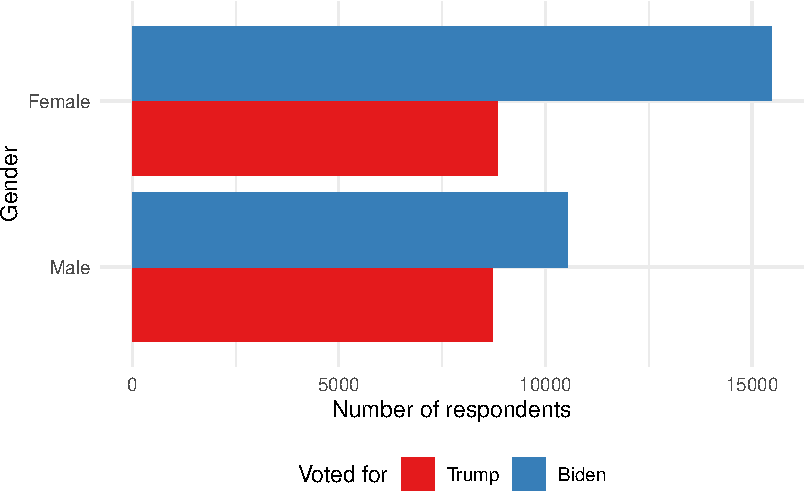
\includegraphics{paper_files/figure-pdf/unnamed-chunk-4-1.pdf}

The gender of survey participants will take values of either ``Male'' or
`` Female''. Out of the 43,547 survey participants, 19,248 were male and
24,299 were female. (Graph 1) shows a bar graph of who respondents vote
for, grouped by gender. It is shown that around 36.4\% of female
participants voted for Trump while 63.6\% voted for Biden. For their
male counterparts, while 45.3\% of male participants voted for Trump,
54.7\% of male respondents voted for Biden. These number indicates that
female voters are more likely to vote for Biden than male voters.
However, this evidence is inconclusive and needs further testing to
conclude the relationship between voters' choice of candidate and their
gender.

\hypertarget{education-level.}{%
\paragraph{Education level.}\label{education-level.}}

Participants' education level is divided into 6 groups: No High School,
High school graduates, some colleges, 2 years of college, 4 years of
college, and post-grad. As shown in the summary statistics, there are
687 out of 43,547 respondents who have not finished high school, and
9810 participants are high school graduates. Additionally, 9290
respondents have some college education, and 4970 have finished 2 years
of college. Out of 43,547 participants, the largest group consists of
individuals with a 4-year college degree, totaling 11,518 respondents.
Finally, the group with the highest level of education is post-grads
with 7272 respondents.

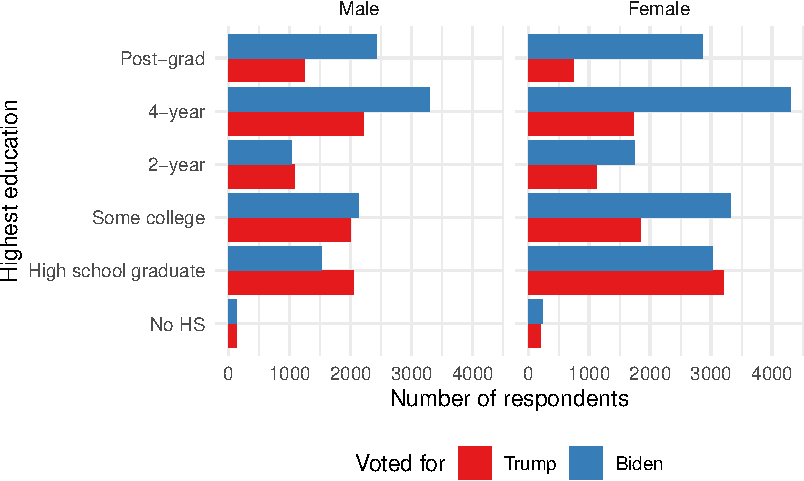
\includegraphics{paper_files/figure-pdf/unnamed-chunk-5-1.pdf}

Graph 2 is a bar graph illustrating the candidates respondents vote for
grouped by gender and education level. Overall, it is found that for the
most part, females with higher education levels are more likely to vote
for Biden while there is no clear trend in male counterparts. It shows
that 51.8\% of male participants with no high school experience voted
for Trump while only 48.2\% voted for Biden. However, 47.5\% of female
respondents with no high school experience voted for Trump while 52.5\%
voted for Biden. The graph also demonstrates that 51.4\% of female high
school graduate participants voted for Trump while 57.3\% of male high
school graduate respondents voted for Trump. Interestingly, it is found
that high school graduates, regardless of gender, are more likely to
vote for Trump than Biden. Furthermore, Graph 2 shows that 51.5\% of
male participants with 2 years of college voted for Trump and 48.9\%
voted for Biden. However, 39.1\% of female participants coming from the
same educational background voted for Trump while 60.9\% voted for
Biden. Additionally, 35.6\% of female respondents with some college
experience voted for Trump while 48.3\% of their male counterparts voted
for Trump. The bar graphs also show that 28.6\% of female respondents
with 4-year college graduates voted for Trump while 40.1\% of the male
participants with the same educational level voted for Trump. Lastly,
34\% of post-grads male participants voted for Trump while only 20.7\%
of the female counterparts voted for Trump. These statistics not only
show that females are less likely to vote for Trump than males but also
show that in general, but it also demonstrates that people with higher
education levels are more likely to vote for Biden.

\hypertarget{model}{%
\section{Model}\label{model}}

The model used to analyze the relationship between the candidate
respondents vote for and voters' demographics is logistics regression.
Logistics regression provides a framework to analyze categorical outcome
variables. Furthermore, logistics regression shows the probability of
the occurrence of an event which is suitable for analyzing binary
variables such as ones in our research. The model that we are interested
in is ( something similar but b3 will be the coefficient of the
interaction terms)

The dependent variable y represents the political preference of the
respondent and is equal to 1 if Biden and 0 if Trump, Gender\_iis the
gender of the respondent with 1 equal to female and 0 if male and
education\_i is the education of the respondent. Additionally,
Gender\_i*education\_i, which is the interaction term of gender and
education, was included to enhance the accuracy of the model and account
for the conditional relationship between the two independent variables.

i is the probability that the ith respondent voted for Biden. Moreover,
it is assumed that the distribution of coefficients B0, B1, and B2 are
normal distributions with a mean of 0 and standard deviations of 2.5.
This assumption is made as the model follows a Bayesian framework which
allows us to incorporate prior information into the model. Assuming that
the distribution of coefficients B0, B1, and B2 follows a normal
distribution allows for a weakly informative prior which implies a
neutrality on the possible value of the coefficients. Mean centering
around 0 implies that there is no bias in the direction of all
coefficients and a standard deviation of 2.5 allows for a moderate level
of variation in the predictor variable. Furthermore, this assumption
also prevents overfitting of the model by constraining the coefficients
to reasonable values.

\hypertarget{result}{%
\section{Result}\label{result}}

\begin{table}
\centering
\begin{tabular}[t]{lc}
\toprule
  & Support Biden\\
\midrule
(Intercept) & \num{0.495}\\
 & (\num{0.085})\\
genderMale & \num{-0.452}\\
 & (\num{0.126})\\
\midrule
Num.Obs. & \num{1000}\\
R2 & \num{0.012}\\
Log.Lik. & \num{-676.067}\\
ELPD & \num{-678.0}\\
ELPD s.e. & \num{5.8}\\
LOOIC & \num{1356.0}\\
LOOIC s.e. & \num{11.6}\\
WAIC & \num{1356.0}\\
RMSE & \num{0.49}\\
\bottomrule
\end{tabular}
\end{table}

\begin{table}
\centering
\begin{tabular}[t]{lc}
\toprule
  & Support Biden\\
\midrule
(Intercept) & \num{-2.239}\\
 & (\num{1.423})\\
genderFemale & \num{1.659}\\
 & (\num{1.454})\\
educationHigh school graduate & \num{1.974}\\
 & (\num{1.457})\\
educationSome college & \num{2.439}\\
 & (\num{1.431})\\
education2-year & \num{2.073}\\
 & (\num{1.401})\\
education4-year & \num{2.710}\\
 & (\num{1.451})\\
educationPost-grad & \num{2.654}\\
 & (\num{1.444})\\
genderFemale × educationHigh school graduate & \num{-1.728}\\
 & \vphantom{1} (\num{1.506})\\
genderFemale × educationSome college & \num{-1.055}\\
 & (\num{1.467})\\
genderFemale × education2-year & \num{-1.352}\\
 & (\num{1.506})\\
genderFemale × education4-year & \num{-0.890}\\
 & (\num{1.494})\\
genderFemale × educationPost-grad & \num{-1.149}\\
 & (\num{1.498})\\
\midrule
Num.Obs. & \num{1000}\\
R2 & \num{0.072}\\
Log.Lik. & \num{-643.222}\\
ELPD & \num{-654.7}\\
ELPD s.e. & \num{9.7}\\
LOOIC & \num{1309.4}\\
LOOIC s.e. & \num{19.3}\\
WAIC & \num{1309.4}\\
RMSE & \num{0.48}\\
\bottomrule
\end{tabular}
\end{table}



\end{document}
